In between the microwave and infrared (IR) frequencies of the electromagnetic (EM) spectrum lies Terahertz (THz) radiation (see Figure \ref{thz_overview}) \cite{zhangIntroductionTHzWave2010}. THz radiation refers to the frequency (wavelength) spectrum ranging from \num{100} \si{\giga\hertz} (\num{3} \si{\milli\meter}) up to \num{10} \si{\tera\hertz} (\num{30} \si{\micro\meter}). 
This part of the spectrum is often referred to as the \enquote{THz gap} (e.g. see \cite{dhillon2017TerahertzScience2017, williamsFillingTHzGap2006, zhangAdvancesTerahertzTechnology2021}), since efficient sources and detectors are still limited compared to adjacent frequency ranges \cite{perkowitzNavigatingTerahertzGap2020}. Over the last decades, significant progress has been made in bridging this gap from both the electronic and photonic side. Advances have been made by extending the high frequency cut-off in purely electronic RF devices, decreasing the lower cut-off frequencies of purely optical IR devices or even by combining the two approaches \cite{preuTunableContinuouswaveTerahertz2011}. A particularly versatile and widely used technique enabled by these developments is THz time-domain spectroscopy (THz-TDS). In THz-TDS, ultrafast femtosecond lasers generate and detect broadband THz pulses, providing direct access to both amplitude and phase information.

Applications of THz-TDS include material characterization \cite{zhangApplicationTHzTDSCharacterization2024}, nondestructive testing cite{kawaseNondestructiveTerahertzImaging2003}, and industrial quality control \cite{prokschaTerahertzInsightsFabric2024, wietzkeTerahertzSpectroscopyPolymers2011}, where broadband signals with high dynamic range are required. For example, THz-TDS enables the detection of intermolecular vibrations in biomolecules \cite{chenLargeOxidationDependence2005,waltherNoncovalentIntermolecularForces2003,fischerTerahertzTimedomainSpectroscopy2005, nagaiDirectEvidenceIntermolecular2005}, or allows monitoring of water content in industrial products \cite{PrinciplesTerahertzScience2009, THzSecurityApplications}. These capabilities make THz systems promising candidates for future compact sensing and imaging solutions \cite{daviesTerahertzSpectroscopyExplosives2008,fischerTerahertzTimedomainSpectroscopy2005,leitenstorfer2023TerahertzScience2023,yangBiomedicalApplicationsTerahertz2016}.

A key enabling device for THz-TDS is the photoconductive antenna (PCA). PCAs are attractive because they can be operated at room temperatures, integrated with fiber-based femtosecond lasers, and fabricated using standard semiconductor processes. Despite these advantages, conventional PCA designs exhibit resonances in the low-frequency regime (typically $< 500$\,\si{\giga \hertz}). These resonances originate primarily from large metallic contact pads and the finite length of the antenna feeding strips needed for PCA operation \cite{nandiErAsInAlGaAsPhotoconductors2021}. In the time-domain, they manifest as oscillations following the main THz pulse. In the frequency domain, they appear as sharp spectral features that dominate the signal and mask higher-frequency components of interest.

The undesired resonances degrade the dynamic range and bandwidth of THz-TDS measurements. Suppressing low-frequency resonances in PCAs is an important prerequisite for improving the broadband performance of THz systems. This thesis addresses this challenge by modifying conventional antenna designs with resistive feeding elements, aiming to achieve flatter frequency responses and reduced time-harmonic oscillations.













% While microwave and infrared sources are able to provide high magnitudes of power at those frequencies, there has been a lack of efficient and feasible high power sources in the THz range \cite{perkowitzNavigatingTerahertzGap2020}. This has led to the common reference to the THz range as the \enquote{THz gap} (e.g. see \cite{dhillon2017TerahertzScience2017, williamsFillingTHzGap2006, zhangAdvancesTerahertzTechnology2021}). THz radiation shows potential in many fields. Thus tremendous efforts have been made in the last two decades to narrow the \enquote{THz gap}. Narrowing the gap has been achieved from both the microwave and the optical side. Advances have been made by extending the high frequency cut-off in purely electronic RF devices, decreasing the lower cut-off frequencies of purely optical IR devices or even by combining the two approaches \cite{preuTunableContinuouswaveTerahertz2011}. Progress has been made not only driven by advances in THz technology but also a wide range of applications. One of the most important techniques using THz radiation is THz Time Domain Spectroscopy (THz-TDS). In many fields such as pharmaceutics \cite{huangProgressApplicationTerahertz2023}, materials sciences \cite{zhangApplicationTHzTDSCharacterization2024}, chemistry \cite{fischerChemicalRecognitionTerahertz2005} and many more (e.g. see \cite{petrovMobileNearfieldTerahertz2023, markelzPerspectiveTerahertzApplications2022,TerahertzSpectroscopyIts2011,kleine-ostmannReviewTerahertzCommunications2011}), THz-TDS has proven to be a valuable technique.

% The THz frequency range exhibits several significant spectral features, including rotational transitions of gas-phase molecules, large-amplitude vibrational modes of organic compounds, lattice vibrations in solids, energy gaps in superconductors and intraband transitions in semiconductors \cite{PrinciplesTerahertzScience2009}. Techniques like THz-TDS exploit these characteristic material responses to probe and analyze the interaction of THz radiation with matter. Compared to the neighboring radio and infrared regions, the THz band exhibits much higher atmospheric opacity due to molecular rotational absorption lines \cite{fedorovPowerfulTerahertzWaves2020}. Water vapor plays a dominant role in attenuating THz radiation as it strongly absorbs energy in this frequency range. The unique spectral line structures of different molecular species allow for their identification within unknown samples. The shapes of these lines offer valuable insight into microscopic processes such as molecular collisions \cite{PrinciplesTerahertzScience2009}.

% Since being introduced THz-TDS has been applied to many materials. Those include biomolecules, medicines, cancer tissue, DNA, proteins and bacteria \cite{chenLargeOxidationDependence2005,waltherNoncovalentIntermolecularForces2003,fischerTerahertzTimedomainSpectroscopy2005}. Here, THz-TDS can deliver valuable information IR spectroscopy cannot. One example is the ability to observe intermolecular vibrations in chemicals and organic molecules where the intramolecular mode appears in the IR region \cite{nagaiDirectEvidenceIntermolecular2005}. Intermolecular vibration studies using THz-TDS are expected to enhance our knowledge of larger biomolecules and the human body \cite{tonouchiCuttingedgeTerahertzTechnology2007}.

% Because of the low photon energy (typically $\sim 1-10$ \si{\milli \electronvolt}) \cite{yangBiomedicalApplicationsTerahertz2016}, THz radiation does not ionize molecules. This makes THz-tomography a great alternative to conventional X-ray techniques, which can break down molecules. THz-TDS can be combined with density functional theory \cite{chenCombinationTerahertzSpectroscopy2022} to study amino acids \cite{liaoAminoacidClassificationBased2023}, peptides \cite{neuTerahertzSpectroscopyTetrameric2019}, drugs \cite{kawaseNondestructiveTerahertzImaging2003} and explosives \cite{daviesTerahertzSpectroscopyExplosives2008}. THz radiation is transparent to most dry dielectric materials due to its relatively long wavelength. THz waves easily penetrate most clothing \cite{prokschaTerahertzInsightsFabric2024} or packaging \cite{wietzkeTerahertzSpectroscopyPolymers2011} material. This makes THz-TDS a valuable technique in security applications, quality and process controls and nondestructive analysis of materials and devices. THz radiations sensitivity to water can be used to control food and agricultural products \cite{afsah-hejriTerahertzSpectroscopyImaging2020}. For example, damage to fruits can be evaluated and the water content in vegetables can be monitored. Within the industrial food sector, compact and high-speed THz cameras capable of providing instant quality control information of products on conveyer belts are needed \cite{THzSecurityApplications}. 

% Examining metamaterials is a subject of great interest as they enable engineered electromagnetic properties not found in naturally occurring materials \cite{lakamanahalliMetamaterialsComprehensiveReview2024}. Metamaterials can exhibit singular electromagnetic properties like a negative refraction index, an effect not found in nature \cite{ramakrishnaPhysicsApplicationsNegative2008}. As THz-TDS provides both amplitude and phase information it can be crucial for understanding the electromagnetic properties and engineering of metamaterials \cite{rouxPrinciplesApplicationsTHz2014}. 

\begin{figure}[!btp]
    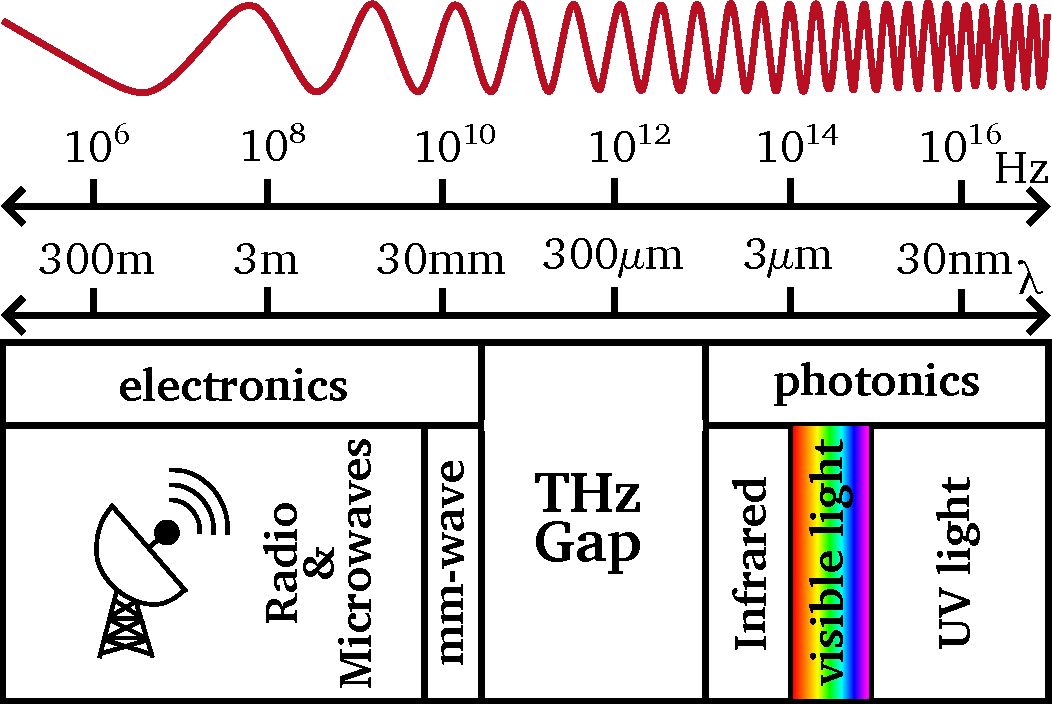
\includegraphics[height=0.4\textwidth]{figures/THz_overview.pdf}
    \centering
    \caption{Schematic diagram depicting the location of the so called THz gap in between electronically and optically generated frequencies.}
    \label{thz_overview}
\end{figure}








